\begin{comment}
--------------------------------------------------------------------------------
\end{comment}
\chapter{Evaluation}\label{ch:eval}


\begin{comment}
--------------------------------------------------------------------------------
\section{Versuchsaufbau [todo]}
\section{Ergebnisse und Auswertung [todo]}
\end{comment}


\begin{comment}
--------------------------------------------------------------------------------
- TODO: Stimmen die 10Hz?
- Start 13:50-23:50, 12:50-20:00 => 10+7 => 17 Stunden
\end{comment}
\section{Batterielaufzeit}

Beim Test der Batterielaufzeit wurden zwei \gls{uwbm} in einem Abstand von \SI{4.7}{\metre} aufgestellt. Beide \gls{uwbm} hatten eine direkte \gls{los} zu einandern. Über den kompletten Zeitraum wurden Entfernungsmessungen mit einer Rate von \SI{10}{\hertz} durchgeführt. Als Testprogramme wurden dabei \textit{DW1000Ranging\_ANCHOR} und \textit{DW1000Ranging\_TAG} aus dem GitHub--Projekt \cite{Trojer2015} verwendet.

Der \Gls{anchor} hatte nach ca. \SI{17}{\hour} seinen Dienst eingestellt, wenig später folgte Ihm der \Gls{tag}. Deutlich höhere Batterielaufzeiten können dadurch erzielt werden, dass die Senderate reduziert wird und die Stromsparfunktionen sowohl des DWM1000 als auch des ATmega328/P genutzt werden.


\begin{comment}
--------------------------------------------------------------------------------
- Versuchsaufbau für die Kalibierung (LGS)
- Ergebnisse
\end{comment}
\section{Kalibierung [todo]}


\begin{comment}
--------------------------------------------------------------------------------
- Mit welchen Einstellungen kommt man auf die Entfernungsmessung?
- Streuung?
- LOS/NLOS {Holz, Bücher, Menschlicher Körper}
	- Welcher Fehler ergibt zwischen LOS/NLOS?
- Wie verändert sich die Genauigkeit der Entfernungsmessung bei einer direkten Sichtverbindung (engl. Line--of--sight (LOS)) und indirekten Sichtverbindung (engl. Non--line--of--sight (NLOS))?
- isaacs2009optimal - Optimal sensor placement for time difference of arrival localization
- Diagramme
	- \cite{kurth2003experimental}
		- Fig. 2: Sample PDFs showing the true ranges associated with 20, 30, and 50 ft measured ranges. (X: true range, Y:count)
		- Fig. 3: The mean true distances to RF tags vs. measured distances (X:measured range, Y: true range)
		- Fig. 4: The variance in true distances to RF tags vs. measured distances (X:measured range (ft), Y: variance (ft^2))
	
- https://matheguru.com/stochastik/standardfehler.html
- https://de.wikipedia.org/wiki/Standardfehler
	
\end{comment}
\section{Entfernungsmessung}

Um die Charakteristik der Entfernungsmessung zu bestimmen, wurde der Versuchsaufbau aus der \figurename~\ref{fig:entfernungsmessung_versuchsaufbau} verwendet. Dabei wird der \Gls{tag} an einem fixen Ort befestigt und die Entfernung zu dem \Gls{anchor} gemessen. Es wurden dabei acht Entfernungen mit einem Abstand von einem Meter gemessen. Zu jeder Entfernung wurden \num{249} Messungen aufgezeichnet. Die tatsächliche Entfernung wird mit einem Laser Entfernungsmesser, der eine Genauigkeit von $\pm$~\SI{2}{\milli\meter} besitzt, bestimmt.

\begin{figure}[ht!]
  \centering
  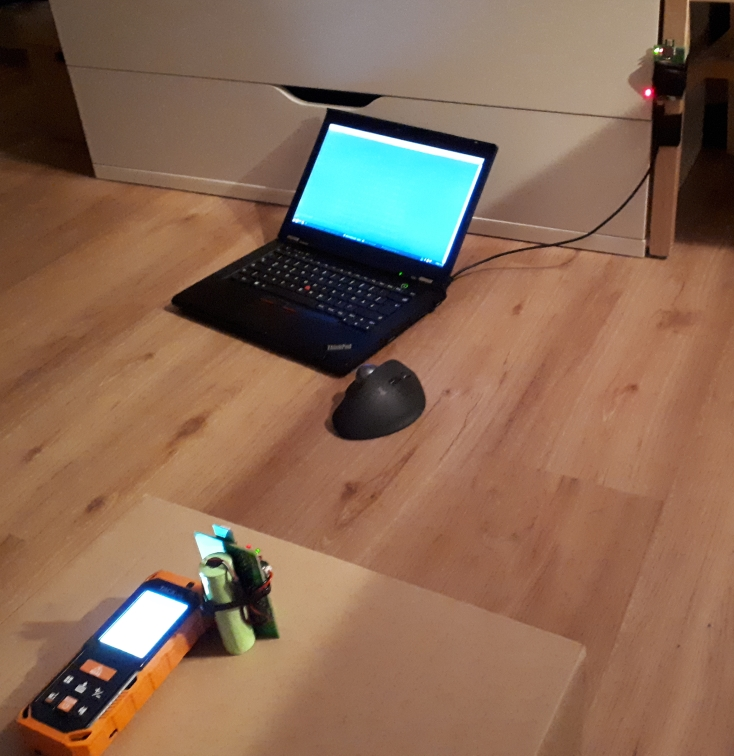
\includegraphics[width=0.5\linewidth]{entfernungsmessung_versuchsaufbau}
	\caption{Versuchsaufbau der Entfernungsmessung.}
	\label{fig:entfernungsmessung_versuchsaufbau}
\end{figure}

Die Ergebnisse der Entfernungsmessung können der \tablename~\ref{tab:entfernungsmessung_stochastik} entnommen werden. Auffällig sind die zum Teil großen Abweichung der Mittelwerte von der tatsächlichen Entfernungen, siehe Entfernung \SI{3}{\meter} und \SI{7}{\meter}. Mit \SI{10}{\centi\meter} sind die größten Ausreißer vom Mittelwert bei \SI{7}{\meter} zu verzeichnen. Die restlichen liegen im Bereich von \SIrange{4}{8}{\centi\meter}. Die Standardabweichung liegt mit \SI{3}{\centi\meter} in einem sehr guten Bereich, siehe auch \figurename~\ref{fig:entfernungsmessung_punktwolke}.

\begin{table}[h!]
	\centering
	\begin{tabular}{||c||c|c|c|c|c|c||}
		\hline
		Entfernung [\si{\meter}] & $\overline{x}_{arithm}$ & $\sigma$ & $\sigma^2$ & $SE_{\overline{x}}$ & Min & Max\\\hline
		\hline
		\num{1.00} & \num{1.0401} & \num{0.0298} & \num{0.0009} & \num{0.0019} & \num{0.96} & \num{1.12}\\\hline
		\num{2.00} & \num{2.0766} & \num{0.0164} & \num{0.0003} & \num{0.0010} & \num{2.03} & \num{2.12}\\\hline
		\num{3.00} & \num{3.1288} & \num{0.0218} & \num{0.0005} & \num{0.0014} & \num{3.07} & \num{3.18}\\\hline
		\num{4.00} & \num{3.9104} & \num{0.0221} & \num{0.0005} & \num{0.0014} & \num{3.86} & \num{3.97}\\\hline
		\num{5.00} & \num{5.0746} & \num{0.0383} & \num{0.0015} & \num{0.0024} & \num{5.00} & \num{5.19}\\\hline
		\num{6.00} & \num{6.0965} & \num{0.0177} & \num{0.0003} & \num{0.0011} & \num{6.05} & \num{6.16}\\\hline
		\num{7.00} & \num{7.1509} & \num{0.0324} & \num{0.0010} & \num{0.0021} & \num{7.08} & \num{7.25}\\\hline
		\num{8.00} & \num{7.9356} & \num{0.0191} & \num{0.0004} & \num{0.0012} & \num{7.89} & \num{7.98}\\\hline
	\end{tabular}
	\caption{Stochastische Eigenschaften der Entfernungsmessungen.}
	\label{tab:entfernungsmessung_stochastik}
\end{table}

\begin{figure}[h!]
  \centering
  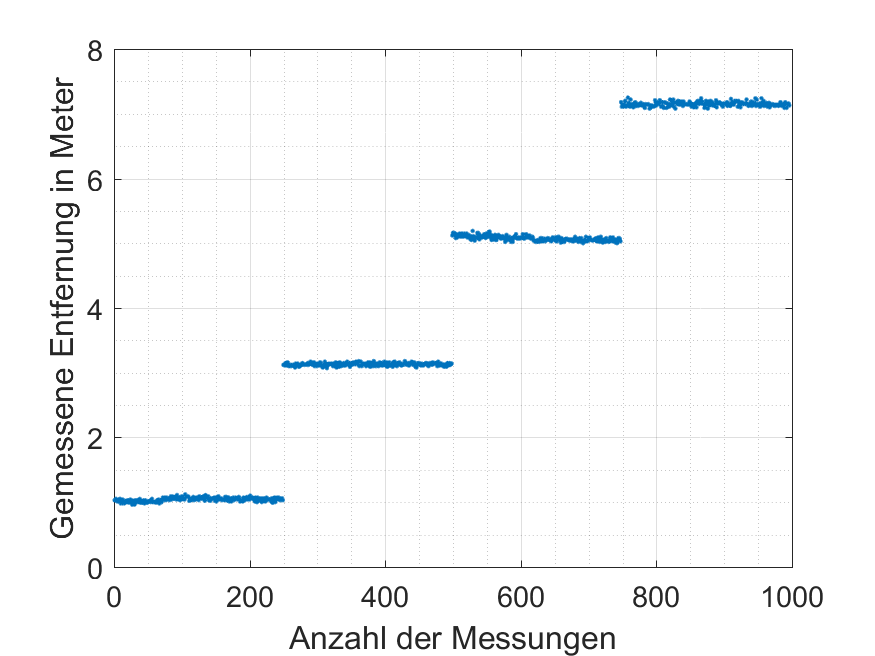
\includegraphics[width=0.5\linewidth]{entfernungsmessung_punktwolke}
	\caption{Verteilung der Messpunkte der ungeraden Entfernungsmessungen.}
	\label{fig:entfernungsmessung_punktwolke}
\end{figure}

In der \figurename~\ref{fig:entfernungsmessung_los_16440} wurden die ungeraden Entfernungsmessungen als Histogramm dargestellt. Gut zu erkennen ist die Normalverteilung der Messwerte um den Mittelwert.

\begin{figure}[h!]
	\centering
	\begin{subfigure}[b]{0.45\textwidth}
		\centering
		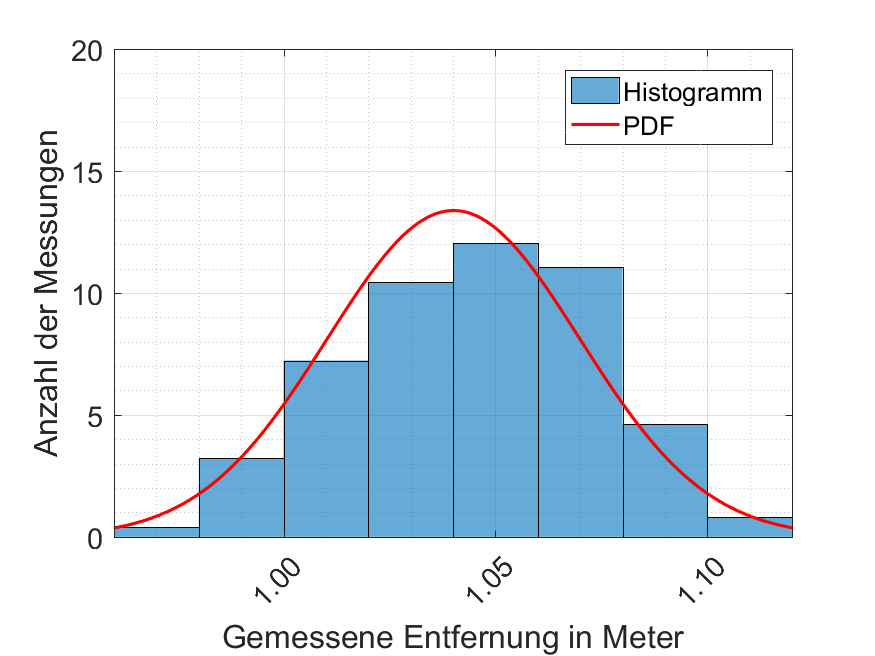
\includegraphics[width=\textwidth]{entfernungsmessung_los_1_16440}
		\caption{1 Meter}
		\label{fig:entfernungsmessung_los_1_16440}
	\end{subfigure}
	\hfill
	\begin{subfigure}[b]{0.45\textwidth}
		\centering
		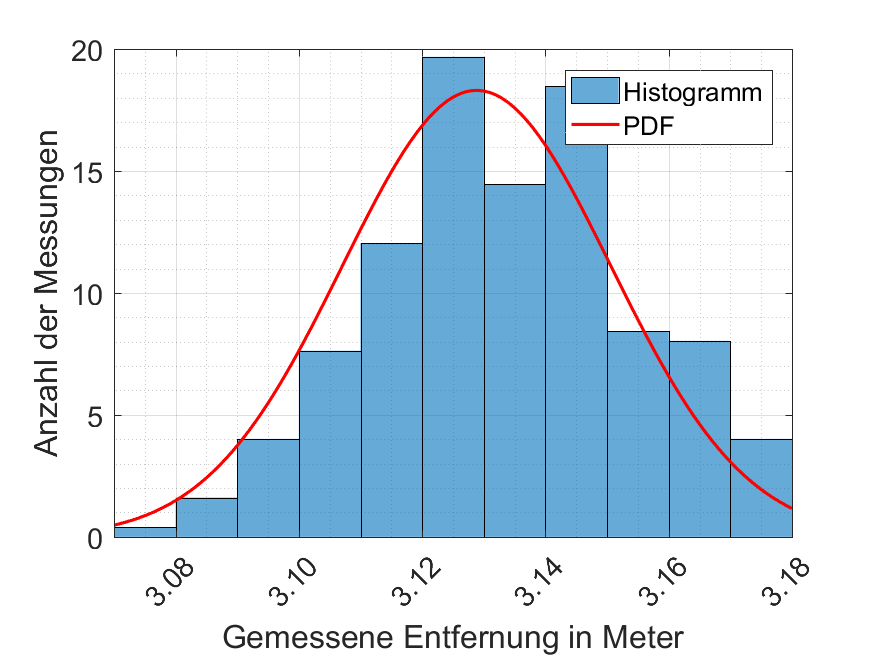
\includegraphics[width=\textwidth]{entfernungsmessung_los_3_16440}
		\caption{3 Meter}
		\label{fig:entfernungsmessung_los_3_16440}
	\end{subfigure}
	\bigskip
	\begin{subfigure}[b]{0.45\textwidth}
		\centering
		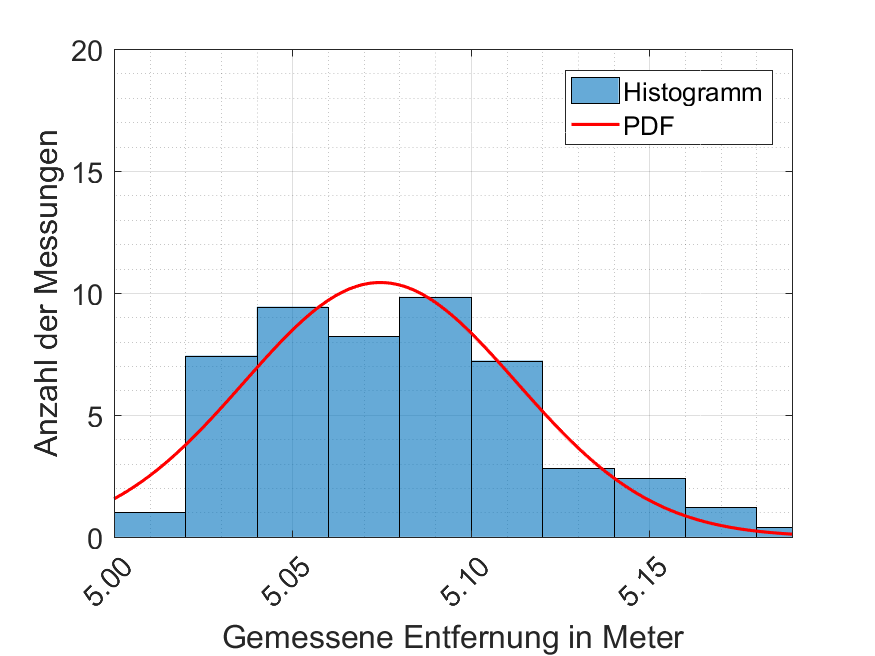
\includegraphics[width=\textwidth]{entfernungsmessung_los_5_16440}
		\caption{5 Meter}
		\label{fig:entfernungsmessung_los_5_16440}
	\end{subfigure}
	\hfil
	\begin{subfigure}[b]{0.45\textwidth}
		\centering
		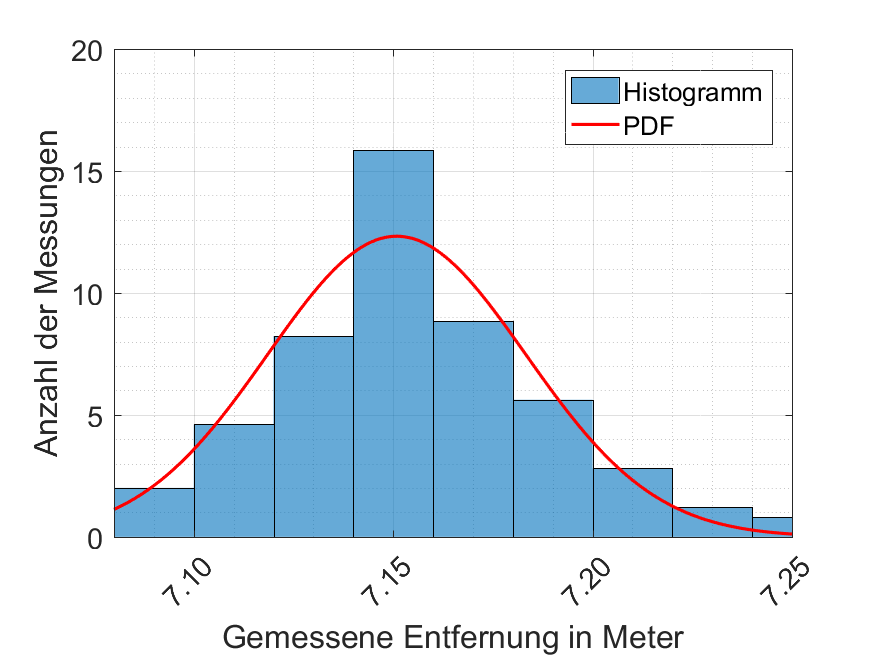
\includegraphics[width=\textwidth]{entfernungsmessung_los_7_16440}
		\caption{7 Meter}
		\label{fig:entfernungsmessung_los_7_16440}
	\end{subfigure}
	\caption{Histogramm und Wahrscheinlichkeitsdichtefunktion der ungeraden Entfernungsmessungen.}
	\label{fig:entfernungsmessung_los_16440}
\end{figure}


\begin{comment}
--------------------------------------------------------------------------------
- Diagramme
	- \cite{kurth2003experimental}
		- Fig. 5: (1) The ground truth path with tags indicated by circles. The numbers indicate how many range measurements were received from each tag over the duration of Test 1. (2) The path estimate from dead reckoning alone. (3) The path estimate from localization using a Kalman Filter. The Filter fuses data from odometry and a gyro with absolute measurements from RF tags to produce this path estimate. Numerical results are given in Table 1. (X: position in x(m), Y: position in y(m), Ground truth path with tag locations, Dead reckoning path, Kalman filter localization path)

		
- Versuchsbeschreibung:
	- Warum wurden die uwbm da platziert wo sie jetzt stehen?
	
\end{comment}
\section{RO-SLAM [todo]}


\begin{comment}
--------------------------------------------------------------------------------
\end{comment}
\subsection{Trajektorie [todo]}


\begin{comment}
--------------------------------------------------------------------------------
\end{comment}
\subsection{Vergleich von MC und SOG [todo]}

